\documentclass[12pt,oneside,openany,letterpaper]{memoir}
\usepackage{graphicx}

\title{Natron For Newbies}
\author{Created By: Matthew Polk\\Rough Draft}
\date{}

\setpnumwidth{3em}
\setrmarg{4em}
\setlength{\cftpartnumwidth}{3em}

% Adjusting the margins. This is subject to change.
\setlrmarginsandblock{1.5in}{1.5in}{*}
\setulmarginsandblock{1in}{1in}{*}

\checkandfixthelayout

% This will rename the title of TOC from "Contents" to something else.
\renewcommand*{\contentsname}{Table Of Contents}

% This will ensure that Table Of Contents page has no page number.
\AtBeginDocument{\addtocontents{toc}{\protect\thispagestyle{empty}}}

%%<=====================================================================>
\begin{document}
\aliaspagestyle{title}{empty}
\maketitle

\newpage

\tableofcontents*
\pagestyle{empty}


\cleardoublepage

%%<====================================================================>
%
% I'm using right now the following books for now as references:
% Nuke 101: Professional Compositor And Visual Effects (A lot of the principles can be applied to natron).
% The Visual Effects Producer
% The VES Handbook of Visual Effects
% The Filmmaker's Guide To Visual Effects
% The Art And Science Of Digital Compositing
% Professional Digital Compositing
% Digital Compositng for Film and Video
\setcounter{page}{1}
\pagestyle{plain}

%%<=================================================================>
\part{Natron Usage}

\chapter{Introduction}
Natron is a free libre (open source) GPL-2.0 licensed compositor styled after nuke. It can be compared to after effects as well, in the sense it makes visual effects for video clips such as a movie.

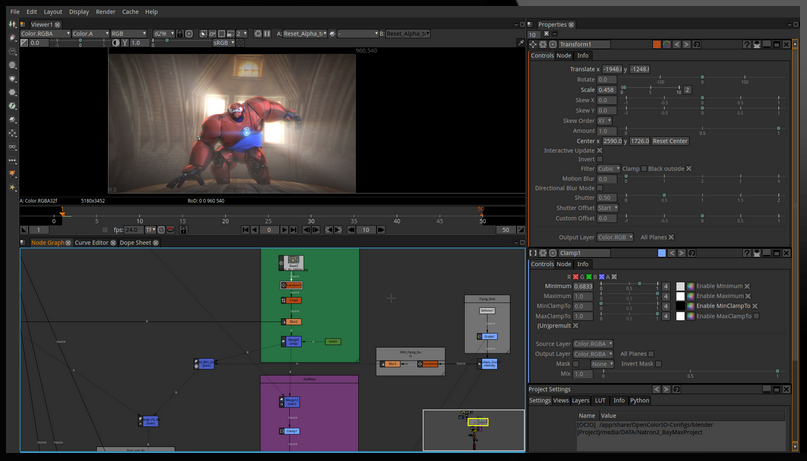
\includegraphics[width=5in,height=5in]{imgs/Natron.png} \\
Image screenshot of natron in action, taken from the natron website.

Head over to https://natrongithub.github.io/ and download it for your OS.



\section{Installing}









\chapter{Nodes}

Nodes. Filter nodes. Combine images. Merging. Parallex. 2D. Rotoscoping. \\
Green Screen, Alpha, PreMultiply. Blue Screen.

RotoPaint. KeyFraming. Snow. Rain. Particles.







\chapter{GMic}
What is GMic.








\chapter{Colours}
RGBA








\chapter{Alpha}
RGBA







\chapter{Input Formats}
Input








\chapter{GUI}
GUI







\chapter{Masks}
Masks







\chapter{Blending Modes}
Modes







\chapter{Closing Thoughts}
Closing Thoughts


%%<=================================================================>
\part{Compositing/VFX Fundamentals}

Compositing

\chapter{References}
Nuke 101. The Visual Effects Producer. \\
The VES handbook of Visual Effects. The Filmmakers guide to visual effects. \\
The Art and Science of digital compositing. \\
Professional Digital Compositing. \\
Digital Compositing For Film.


%%<=================================================================>
\part{ Extending Natron}
Extending

\chapter{Python API}
Python

\chapter{GLSL}
GLSL

\chapter{Command Line}
Command Line


%%<=================================================================>

\part{Other}
Other.



%%<=================================================================>

That's all folks!


\end{document}
